\begin{center}
	\Huge
	Differentialligninger i Maple
\end{center}

\section*{Hældningsfelter}
\stepcounter{section}

Vi genopfrisker, hvad vi mener med et hældningsfelt for en differentialligning. Lad os betragte en differentialligning
\begin{align*}
	y' = f(x,y). 
\end{align*}
Vi definerer et \textit{linjeelement} til differentialligningen som et punkt i $(x,y)$-planet samt hældningen af løsningen til differentialligningen i dette punkt. Vi noterer et linjeelement som
\begin{align*}
	(x_0,y_0;a),
\end{align*}
hvor $(x_0,y_0)$ er punktet i $(x,y)$-planen og $a = y'(x_0)$ for en løsning $y(x)$ til differentialligningen. 
\begin{exa}
	Vi betragter differentialligningen 
	\begin{align*}
		y' = \frac{x}{y^2}.
	\end{align*}
	Så længe $y\neq 0$, så kan vi bestemme linjelementer for løsningskurver til denne differentialligning. Vælger vi punktet $(4,2)$, så kan vi finde linjeelemenentet i dette punkt ved at indsætte i 
	differentialligningen:
	\begin{align*}
		y' = \frac{4}{2^2} = 1,
	\end{align*}
	og et linjeelement til denne differentialligning lyder
	\begin{align*}
		(4,2;1).
	\end{align*}
	Dette linjeelement er illustreret på Fig. \ref{fig:linjeelement}.
	\begin{figure}[H]
		\center
		\begin{tikzpicture}
			\begin{axis}[
			axis lines = middle, 
			xmin = -1, 
			xmax = 5,
			ymin = -1,
			ymax = 5, 
			xlabel = {$x$},
			ylabel = {$y$}
			]
				\addplot[color = blue, thick, domain = 3.5:4.5] {x-2};
				\filldraw[color = purple] (axis cs:4,2) circle (2pt);
				\node at (axis cs: 4.4,1.6) {(4,2)}; 				
			\end{axis}
		\end{tikzpicture}
		\caption{Linjeelementet $(4,2;1)$}
		\label{fig:linjeelement}
	\end{figure}
\end{exa}
Sammensætter vi mange af disse linjeelementer så får vi et hældningsfelt. I Maple gøres dette ved følgende kommando:
\begin{align*}
	&\texttt{restart}\\
	&\texttt{with(Gym):}\\
	&\texttt{linjeelementer(y=f(x,y),y,x=xmin..xmax,y=ymin..ymax)}	
\end{align*}
Lad os betragte et eksempel:

\begin{exa}
	Vi ser på differentialligningen
	\begin{align*}
		y' = \frac{x}{y^2}.
	\end{align*}
	Vi ønsker at bestemme et hældningsfelt for denne differentialligning for $x\in [-8,8]$ og $y\in [-8,8]$. Vi skriver følgende i Maple:
	\begin{align*}
		&\texttt{restart}\\
		&\texttt{with(Gym):}\\
		&\texttt{linjeelementer(y=x/y\string^2,y,x=-8..8,y=-8..8)}
	\end{align*}
	Dette giver os hældningsfeltet på Fig. \ref{fig:heldning}
	\begin{figure}[H]
		\center		
		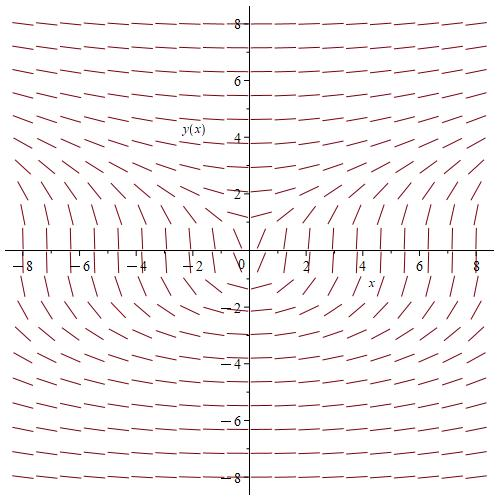
\includegraphics[width=0.7\textwidth]{Billeder/linjeelement.jpg}
		\caption{Hældningsfelt for differentialligningen $y' =x/y^2$}
		\label{fig:heldning}
	\end{figure}
\end{exa}

\section*{Løsning af differentialligninger}
\stepcounter{section}

Vi kan også løse differentialligninger i Maple. Har vi en differentialligning
\begin{align*}
	\frac{dy}{dx} = f(x,y), 
\end{align*}
så kan den løses i Maple med følgende syntaks:
\begin{align*}
	&\texttt{restart}\\
	&\texttt{with(Gym):}\\
	&\texttt{dsolve(y' = f(x,y))}
\end{align*}
Dette giver den fuldstændige løsning. Har vi ydermere en begyndelsesværdi $y_0 = y(x_0)$, hvor $y(x)$ er en løsning til differentialligningen, så kan vi løse begyndelsesværdiproblemet med følgende.
\begin{align*}
	&\texttt{restart}\\
	&\texttt{with(Gym):}\\
	&\texttt{dsolve([y' = f(x,y),y(x\string_0)=y\string_0])}
\end{align*}
Lad os betragte et eksempel.
\begin{exa}
	Vi ser på differentialligningen
	\begin{align*}
		y' = x^2 +y
	\end{align*}
	Vi finder den fuldstændige løsning ved
	\begin{align*}
		&\texttt{dsolve(y' = x\string^2+y)},
	\end{align*}
	og vi får løsningen
	\begin{align*}
		y(x) = -x^2 - 2x - 2 + ce^x.
	\end{align*}
	Har vi ydermere begyndelsesbetingelsen $y(0) = 10$, så skrives
	\begin{align*}
		&\texttt{dsolve([y' = x\string^2+y,y(0)=10])},
	\end{align*}
	og vi får den partikulære løsning
	\begin{align*}
		y(x) = -x^2 - 2x - 2 + 12e^x.
	\end{align*}
\end{exa}	


\section*{Opgave 1}
\begin{enumerate}[label=\roman*)]
	\item Bestem et linjeelement til differentialligningen 
	\begin{align*}
		y' = xy+y^2
	\end{align*}
	i punkterne $(-2,4)$ og $(10,3)$.
	\item Bestem et linjeelement til differentialligningen 
	\begin{align*}
		y' = \frac{y}{x}
	\end{align*}
	i punkterne $(1,0)$ og $(-5,7)$.
\end{enumerate}

\section*{Opgave 2}
\begin{enumerate}[label=\roman*)]
	\item Bestem et hældningsfelt til differentialligningen
	\begin{align*}
		y' = 7y
	\end{align*}
	for $(x,y)\in [0,5]\times [0,5]$.
	Vurdér, om funktionen $y(x) = e^{-4x}$ kan være en løsning til differentialligningen. 
	\item Bestem et hældningsfelt til differentialligningen
	\begin{align*}
		\frac{dy}{dx} = \frac{x^2}{y^3}.
	\end{align*}
\end{enumerate}

\section*{Opgave 3}
\begin{enumerate}[label=\roman*)]
	\item Bestem en partikulær løsning til differentialligningen 
	\begin{align*}
		y' = \cos(x)\sin(x),
	\end{align*}
	der går gennem punktet $(\pi,4)$. 
	\item Bestem en partikulær løsning til differentialligningen 
	\begin{align*}
		y' = \sqrt{x}\cdot y^2,
	\end{align*}
	der går gennem punktet $(0,4)$.
	\item Bestem en fuldstændig løsning til differentialligningen
	\begin{align*}
		\frac{dy}{dx} = \cos(xy)
	\end{align*}
	\item Bestem en partikulær løsning til differentialligningen
	\begin{align*}
		\frac{dy}{dx} = y\cdot \sqrt{\frac{1}{x}},
	\end{align*} 
	der går gennem punktet $(1,1)$.
\end{enumerate}

\section*{Opgave 4}
Lad $B(x)$ betegne antallet at bakterier i mia. i en koloni som funktion af antal timer $x$ og lad $B'$ betegne bakterievæksten. Det maksimale antal bakterier i kolonien er 16.7 mia. I en model er bakterievæksten proportional med produktet mellem bakterieantallet og forskellen mellem bakterieantallet og det maksimale antal bakterier.
\begin{enumerate}[label=\roman*)]
	\item Opstil en differentialligning, der beskriver bakterievæksten.
	\item Udnyt, at antallet af bakterier, når der er 1 mia bakterier, tiltager med 130 mio bakterier i timen til at bestemme proportionalitetsfaktoren.
	\item Udnyt, at der til tidspunktet $x_0 = 0$ er 2.1 mia bakterier til at bestemme en partikulær løsning til differentialligningen.
	\item Bestem, hvornår der vil være 12 mia. bakterier i kolonien.
\end{enumerate}
